%!TEX root = ./main.tex
%
% This file is part of the i10 thesis template developed and used by the
% Media Computing Group at RWTH Aachen University.
% The current version of this template can be obtained at
% <http://www.media.informatik.rwth-aachen.de/karrer.html>.
\chapter{Hardware Prototype and Software Development}
\label{Hardware Prototype and Software Development} 
\index{hardware prototype}
In this chapter we will present the hardware prototypes. Furthermore, we describe the disadvantages and improvements of former iterations leading to the final prototype. The software implementation is described afterwards.

\section{System Design}
\mnote{MSP430 for first prototype}All prototypes presented here are using pinstripe, a fabric with separated conductive lines. For the first prototype we used the Texas Instruments MSP430G2452 microcontroller. Each row and column of the pinstripe fabric has to be connected to a \emph{digitalRead} pin of the micro-controller. The \index{MSP430G2452}MSP430 controller has 16 of these pins but only 14 can be used since two pins are used for serial communication. This results in a matrix resolution of 7 by 7 at maximum. 
\\ \\
\index{resolution}\myDefBox{Resolution in pinstripe context}{When speaking of a certain resolution of our prototype, we talk about the number of connected rows and columns. \index{pinstripe fabric}Since the pinstripe fabric is of a fixed size (3mm conductive material and 3mm spacing). Therefore the higher the resolution the larger the prototype gets. }

We use the \index{TI EK-TM4C1294XL}TI EK-TM4C1294XL for the advanced prototypes. This board has the ability to connect more than 40 pins for \emph{digitalRead} to operate a 20 by 20 sensor. The board is connected to a Computer via USB for serial communication. \index{serial communication}Short range wireless communication with Bluetooth is added to the final prototype.\\

\mnote{Programming Environment: \index{Enargia}Energia IDE and \index{Processing}Processing to gather, send and process input data}For programming the micro-controller we are using the \href{http://energia.nu}{Energia IDE}\footnote{http://energia.nu}. It is an easy to use IDE to upload programs to the TI micro-controller. The micro-controller itself is solely responsible for sending the data of the sensor to the computer via serial communication. Meaning that it tests a pin against ground for each other line and column. A \emph{1} is written to the serial-port when it is connected to another line or column and \emph{0} otherwise. This is done for each pin where \emph{numberOfPintripes} is the number of all lines and columns. For each prototype an integer array is declared and can easily be commented and uncommented depending on the prototype. The pin numbers are sorted such that the first pins correspond to the x-axis and the last pins to the negative y-axis. After all pins were tested we send a line-break to determine the end of the current input.\\ \\

We are using \href{http://processing.org}{Processing}\footnote{http://processing.org}, a Java based IDE, to structure the input stream from the microcontroller for further analyses. This includes several programs which either display the raw touch points for debugging purpose or filter and display the sensor data. The changes of software are described along with each hardware iteration. 

\section{Early Testing}
After deciding to go for the resistive approach, the essential challenge is to find a spacing material with certain characteristics. The material should
\index{material requirements}
\begin{itemize}
\item be flexible by means of being wearable
\item reliably separate the pinstripe fabric while no touch is intended
\item and concede easily when intended force is applied.
\end{itemize}
We glued both layers of the pinstripe fabric to sheets of paper to eliminate stretching and curling of the fabric. We cut equidistant circular holes to provide space for the pinstripe layers to connect. To display where a touch is present, we created a simple program with Processing. Some of the materials we tested are shown in figure~\ref{fig:earlymats} but were not well suited as foam which we used for the latest prototypes.
\begin{figure}
\includegraphics[scale=0.05]{images/earlytesting.jpg}
\caption{Materials used for testing (polyester grid fabric, plastic latticework, jeans with fly screen, and microcellular rubber).}
\label{fig:earlymats}
\end{figure}

\section{The Prototype}

\index{spacing material}The prototype uses a 3 mm thick layer of foam, coated with a thin layer of cotton, for spacing. Foam has the properties we need to separate the pinstripe layer while no force is applied and yields rather easily when the user presses on it. Another positive feature is the increased resistance to unintended pressure caused by bending or accidental contact with the sensor.
\\
We use a laser cutter to cut equidistant holes out of the foam to allow the pinstripe layers to connect. This procedure leaves enough foam between the holes to retain the properties we need. \\ \\
\mnote{Issues with flexibility and translatory movement}Another problem we have to address is the stretchability and the translatory movement of the fabrics. Each time the user performs a gesture the upper layer moves in the respective direction due to the friction between the operating finger and the surface. This causes the the pinstripe fabric to shift such that the conductive stripes are not aligned to the holes properly, resulting in the prototype to stop working. When we started testing we used needles, clips, and nails to fix the materials to each other. Not only that these methods are not well suited for wearablity, also fixing the materials exclusively at the edges is not sufficient.  The flexibility of the pinstripe fabric can causes shifts that we want to eliminate. 
\\ \\
\mnote{Vliesofix for fixating the components of the prototype} To deal with the issues described above we use Vliesofix. Vliesofix is an adhesive on paper which can be ironed on textile. The paper can be removed afterwards and another fabric can be ironed to the corresponding textile. This results in an extensive adhesive area between two fabrics. The application of Vliesofix not only resolves the translatory movement but also the curling of the pinstripe fabric.
\\ \\
We decide two to prototypes with different dimensions shown in figure~\ref{fig:bothprototypes}. The first prototype has a resolution of 14 by 14 pinstripes and the second prototype has a resolution of 20 by 20. Since the procedure of making the prototypes is similar we only describe its building procedure for the smaller one. 
\begin{figure}
\includegraphics[scale=0.06]{images/bothprototypes.jpg}
\caption{The 14 by 14 pin prototype on the left and 20 by 20 pin prototype on the right}
\label{fig:bothprototypes}
\end{figure}
\\
We start by cutting out a 137 by 125 cm piece of the 3 mm foam using the laser cutter. Then we cut out two sheet of Vliesofix with the corresponding dimensions and proceed by ironing them on both sides of the foam. This has to be done carefully since applying heat for too long can cause the foam to melt. As a result, the foam loses the desired properties to a certain degree. When removing the iron too soon the Vliesofix might not be adhesive enough. 
\\ \\
\mnote{Assembling the prototype}Once the material is cooled off we can remove the paper of the Vliesofix. We proceed with cutting the holes in the foam with the Vliesofix. Making the laser cutter cut more rows and columns of holes ensures that the resistance of the foam is the same throughout the touch sensitive area. Otherwise more force is needed at the edges than the center. 
\\
\index{Vliesofix}To prepare the two pinstripe layer to adhere it to the foam we again use Vliesofix first for preventing the fabric from curling and easy stretching. We do so before cutting out the pinstripe to make handling the fabric easier. Note that, while using Vliesofix with the pinstripe fabric, it is even more important to not apply heat for too long. When the Vliesofix becomes liquid it gets soaked into the fabric. In some cases we ascertained that for this reason the conductivity of the pinstripes gets lost in some places. This immediately renders the sensor useless. Apart from that we do not remove the paper of the Vliesofix at this point.
\\ \\
We proceed with attaching the pinstripe layers to the foam. The stripes of each layer must be perpendicular to one another. Then we iron the untreated side of the  one pinstripe fabric to the foam and after cooling off the other pinstripe to the other side.  We have to make sure that the conductive stripes and the holes in the foam are aligned properly. Now we can remove the paper from the pinstripe fabric. The arrangement of the materials is shown in figure~\ref{fig:matorder}.\\
\begin{figure}
\includegraphics[scale=0.05]{images/matorder.jpg}
\caption{The layer of the prototype in correct order with Vliesofix already applied to the lower pinstripe fabric and jeans as potential upper layer.}
\label{fig:matorder}
\end{figure}
After that we iron a corresponding piece of polyester on the upper side of the sensor to reduce the friction between the finger and treated pinstripe layer. The last step is to connect the sensor to the micro controller. Furthermore we connect a HC06  Bluetooth module for wireless data stream. The power source can either be a computer or an battery pack which are connected by a micro USB cable.
 
\section{The Software}
\index{software}
The software is divided into two parts, the code running on the micro controller and the application running on the computer. The code for the micro controller is straight forward. We define a one dimensional array for each prototype in which the pin numbers are stored such that the first half of the array denotes the horizontal x-axis starting from left to right and the second half the vertical y-axis starting from top to bottom. Now we can check each pin of the array respectively if it is connected to ground. This means that the conductive stripe connected to that pin has a connection to another stripe and a \emph{1} is sent via the serial communication and a \emph{0} otherwise. The line break after the \emph{for} loop lets us determine if a complete input set is received.

\mnote{Receiving the data via serial communication in Processing}In Processing we read the data from the serial communication and store it in a buffer including the time stamp.  If at least one \emph{1} per data set is read, we consider it to be a touch. Sometimes the contact of the pinstripe layer is lost while performing a gesture due to insufficient pressure or a undersized locating surface of the operating finger. Therefore we implemented a threshold in which we can read only \emph{0} without the touch phase to end. This threshold is reset anytime a \emph{1} is read. The raw data is logged for potential analyses. \\ \\
\index{filter algorithm}\mnote{Use a filter algorithm to reduce a set of touch points to one point}Since more than one vertical and horizontal pinstripe can be connected at the same time we apply a filter algorithm. This algorithm takes all x-coordinates and calculates the average and the same for the y-coordinates. The resulting triple composed of the coordinate and the time stamp is added to an \emph{Arraylist} buffer. This is done for all input sets except for all those, which only consist of \emph{0's}. There are two reasons for filtering the input data. The first is the resilience to noise caused by unintended connections or slow separation of the pinstripe layers. The second reason is fact that it is easier for implementing gesture recognition. Apart from this the user intends to press only one point at the sensor.
\\
When a gesture starts we take the coordinates and subtract them from all filtered coordinates of this gesture. Therefore every gesture starts at $(0,0)$ regardless where it is performed on the sensor. This is done for the graphical representation of the strokes and will be useful later on.
\\ \\
\index{mark-based gesture recognition}\mnote{Implementing mark-based gesture recognition}The next step is to actually recognize easy strokes performed on the prototype.  Since our prototypes have a rather low resolution compared to typical touch input devices we focus on rather simple unistroke gestures. These mark-based gestures are shown in figure \ref{fig:markBasedGestures}. We extend this gestures set by adding 5 gestures. These gestures are a tab and for each swipe gesture we expand it with a swipe in the opposite direction. This leads to a gesture set with 17 simple gestures. \\
\begin{figure}
 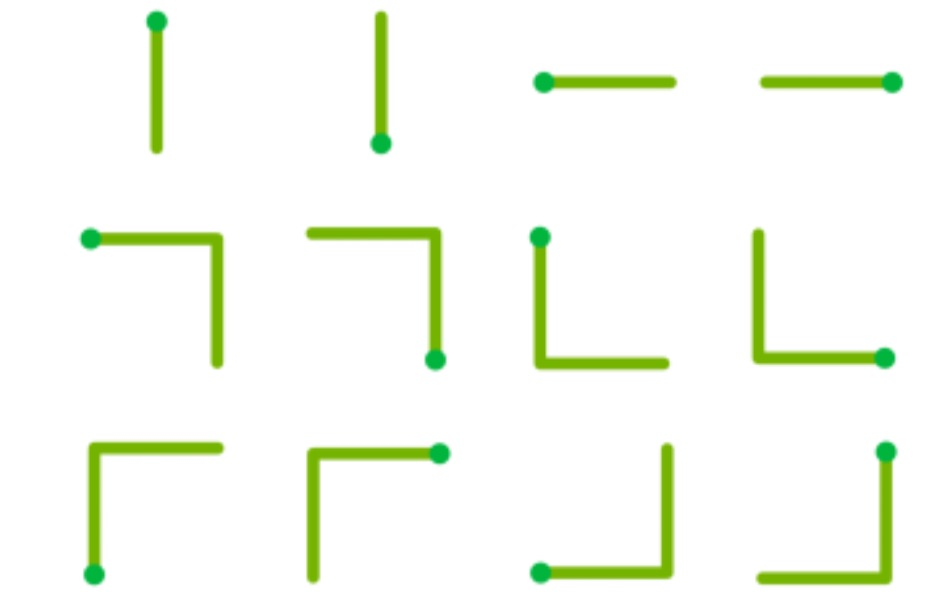
\includegraphics[scale=0.25]{images/markBasedGestures.jpg}
 \caption{Mark-based gestures. Gestures start at the dots. \cite{Bragdon}}
 \label{fig:markBasedGestures}
 \index{mark-based gestures}
 \end{figure}Our gesture recognition works as follows. First of all we do not recognize in real-time. We analyze all filtered points, stored in the buffer, after a gesture is considered finished.  Then the algorithm works as follows.
\begin{tt}
\begin{itemize}
\item check for tap
	\begin{itemize}
		\item return $true$ if the size of the buffer is $1$ 
		\item return $true$ if all coordinates have a $distance$ smaller or equal to $1$ respectively and the time elapsed is smaller than 200 milliseconds
		\item else check for other gestures
	\end{itemize}
\item check for swipe
	\begin{itemize}
	\item assume there is a swipe with the first and the last item of the buffer as terminal points
	\item calculate the $length$ of the line
	\item return $false$ if the $length$ is smaller than $3$
	\item for all other points calculate the $distanceToLine$ 
	\item return $false$ if at some index the $distanceToLine$ is greater than $1$
	\item else determine the direction of the swipe and return $true$
	\end{itemize}
\item check for angle
	\begin{itemize}
	\item check if there is a line between the point at $ index - 1$ and last point in the buffer under the exact same conditions applied for swipe
	\item return $false$ if at some index the $distanceToLine$ is greater than $1$
	\item calculate the directions of both lines and return $true$
	\end{itemize}
\item end of checking 
\end{itemize}
\end{tt}
This algorithm classifies each gesture as a tap, swipe, angle, or no gesture. In combination with the directions we calculate for each swipe we can distinguish between all 16 mark-based gestures. The orientation of a line is mapped to one of the four directions up, left, right, or down. Therefore our prototype is resilient to a certain degree of input error. With less effort we can further extend the gesture set by distinguish more directions. 
\\ \\
\index{free-form gesture recognition}\index{1\$ recognizer}\mnote{Using 1\$ Unistroke Recognizer for complex gestures}When testing our gesture recognizer with our current prototypes we observe an almost 100\% recognition rate. Based on this finding we decide to go beyond simple mark-based gestures and continue with recognizing  more complex gestures. Therefore we make use of the 1\$ Unistroke Recognizer by \cite{Wobbrock}. This is an easy to implement recognizer which does not require any training data. Providing a template for each gesture is sufficient. A template is an array of consecutive pairs of coordinates. We can pass the coordinates in the filtered buffer straight to the 1\$ recognizer.
\\
This recognizer is orientation independent. Meaning for the marked-based gestures that, without further analysis of orientation, we can only distinguish between a swipe, an angle to the right, and an angle  to the left. However, we can recognize a set of free-form gestures shown in figure \ref{fig:freeFormGestures}.
\begin{figure}
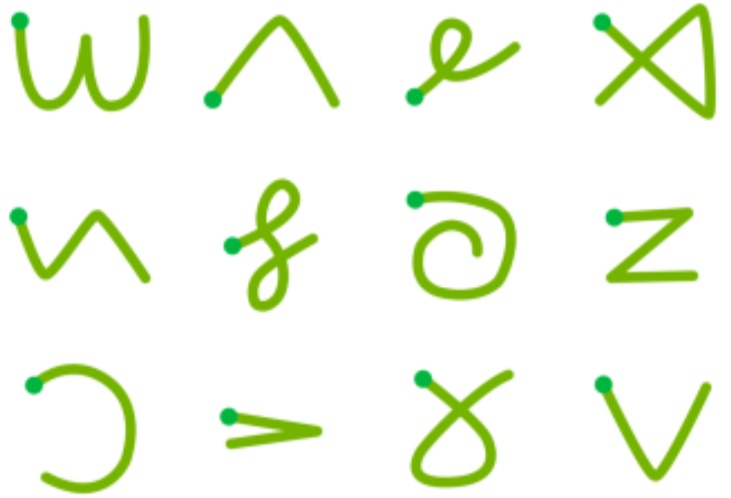
\includegraphics[scale=0.3]{images/freeFormGestures.jpg}
\caption{Free-form gestures \cite{Bragdon}}
\label{fig:freeFormGestures}
\index{free-form gestures}
\end{figure}


\chapter{System Evaluation}
\index{system evaluation|}
\label{evaluation}
In this chapter we will evaluate the robustness of our prototype in different extreme conditions.\mnote{Testing the 14 by 14 prototype} We will take a closer look at the performance of the 14 by 14 prototype. Since the prototype is designed as a wearable, we are interested in its behavior under changing conditions. These conditions are composed of softness, curvature, and friction.

\section{Physical Limitation Study}
\index{study condition}\mnote{Independent variables: friction, softness, looseness, and curvature}The human body is in motion almost all the time and the clothes we are wearing are not fixed to the skin. This \emph{looseness} and the changing subsurface are variables that influence the performance of our prototype. Another variable is the \emph{friction} of the overlaying common everyday fabrics. Depending on the fabric and method of fashioning, it can, more or less likely, happen that the user slips of the touch-sensing area, or experiences an unpleasant feeling in the operating finger. Furthermore the \emph{softness} of the underlying surface may influence the performance of our prototype. The amount of muscles, adipose tissue, and so forth also differs from human to human. This, in the first place, affects the pressure needed by the user. Then there are the different levels of \emph{curvature}. Our prototype has flexible spacing-material to separate the pinstripe layer. After a certain amount of bend the material starts creasing, causing some permanent contacts. In this study we will test our prototype in conditions which aim to simulate the in field scenarios. To test to which degree of bend the prototype breaks we used different foams with fixed thickness and different density.

\section{Experiment Setup}
\mnote{The conditions}The conditions and their levels are shown in table \ref{table:conditions}. This leads to 18 combinations in total. For softness we have chosen the solid surface as a baseline. The soft foam with a density of 1000m$^3$ was considered similar enough to the soft spots on the human body. Curvature has a flat surface as baseline, 66mm diameter curvature, and 53mm diameter as fringe condition. Prior testing has proven that going below 53mm leads to permanent contact due to a kink in the spacing material. Friction is depending on the materials used for the outer layer of the sensor and the clothing, respectively. We have decided to test cotton, jeans and rib knit cotton shown in figure~\ref{fig:mats}. They have distinct surface characteristics and behavior when moving across with the finger. \\ \\\begin{figure}
\includegraphics[scale=0.05]{images/mats.jpg}
\caption{The materials used in the experiment (cotton, jeans, and rib knit cotton).}
\label{fig:mats}
\end{figure}\begin{table}
\begin{tabular}{|c|c|}
  \hline
  \textbf{variable}& \textbf{levels} \\
  \hline
  curvature & 3 (flat, 66mm diameter, 53mm diameter) \\
  \hline
  softness &2 ( solid, foam 1000m$^3$ density) \\
  \hline
  friction & 3 (cotton, jeans, rib knit cotton) \\
  \hline
\end{tabular}
\caption{Variables and their levels.}
\label{table:conditions}
\end{table}\mnote{System setup}The users sat in front of a desk on which the conditions were prepared consecutively. The sensor was fixed to the surface below and the overlying fabric was fixated in the corners with pins. Nevertheless, there is still a certain amount of movement due to the flexibility of the overlying fabrics. For the curvature, we used aerosol cans with 53mm diameter and 66mm diameter. We fixated the aerosol cans with stands made with a laser cutter. To achieve the curvature with the foam, we used a book and wrapped the foam around the cover and hemmed it in a vise. A GoPro camera was placed such that each setup was captured obliquely from above as shown in figure \ref{fig:topview} and figure \ref{fig:53mmtopview}. The observer sat next to the participant ready to make notes and start or stop recording the setup. The user cannot see the output on the screen. Additionally, our program created two log-files for each condition. One logged the filtered data and one the raw sensor data. Both files logged the time stamps of each data point.\\ \\\begin{figure}
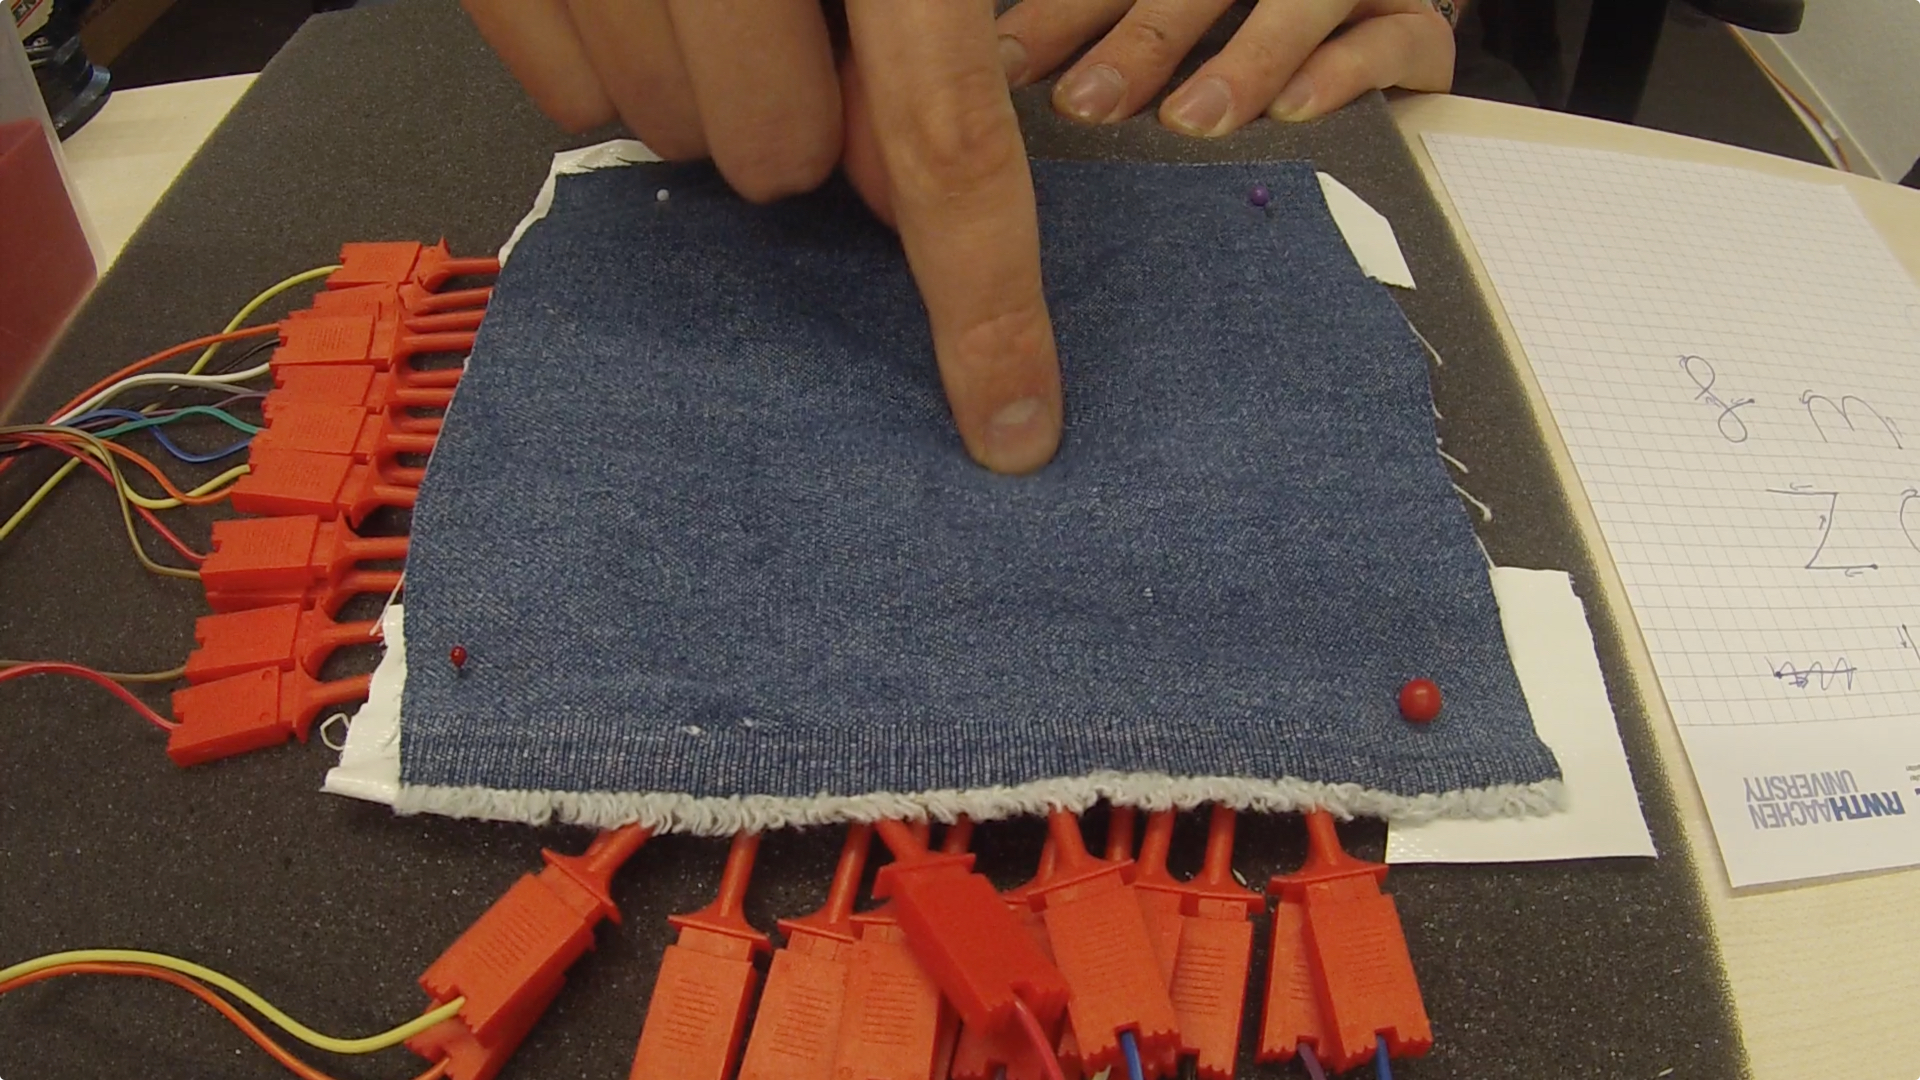
\includegraphics[scale=0.15]{images/topview.jpg}
\caption{Condition: flat, jeans, foam, on the table}
\label{fig:topview}
\end{figure}\begin{figure}
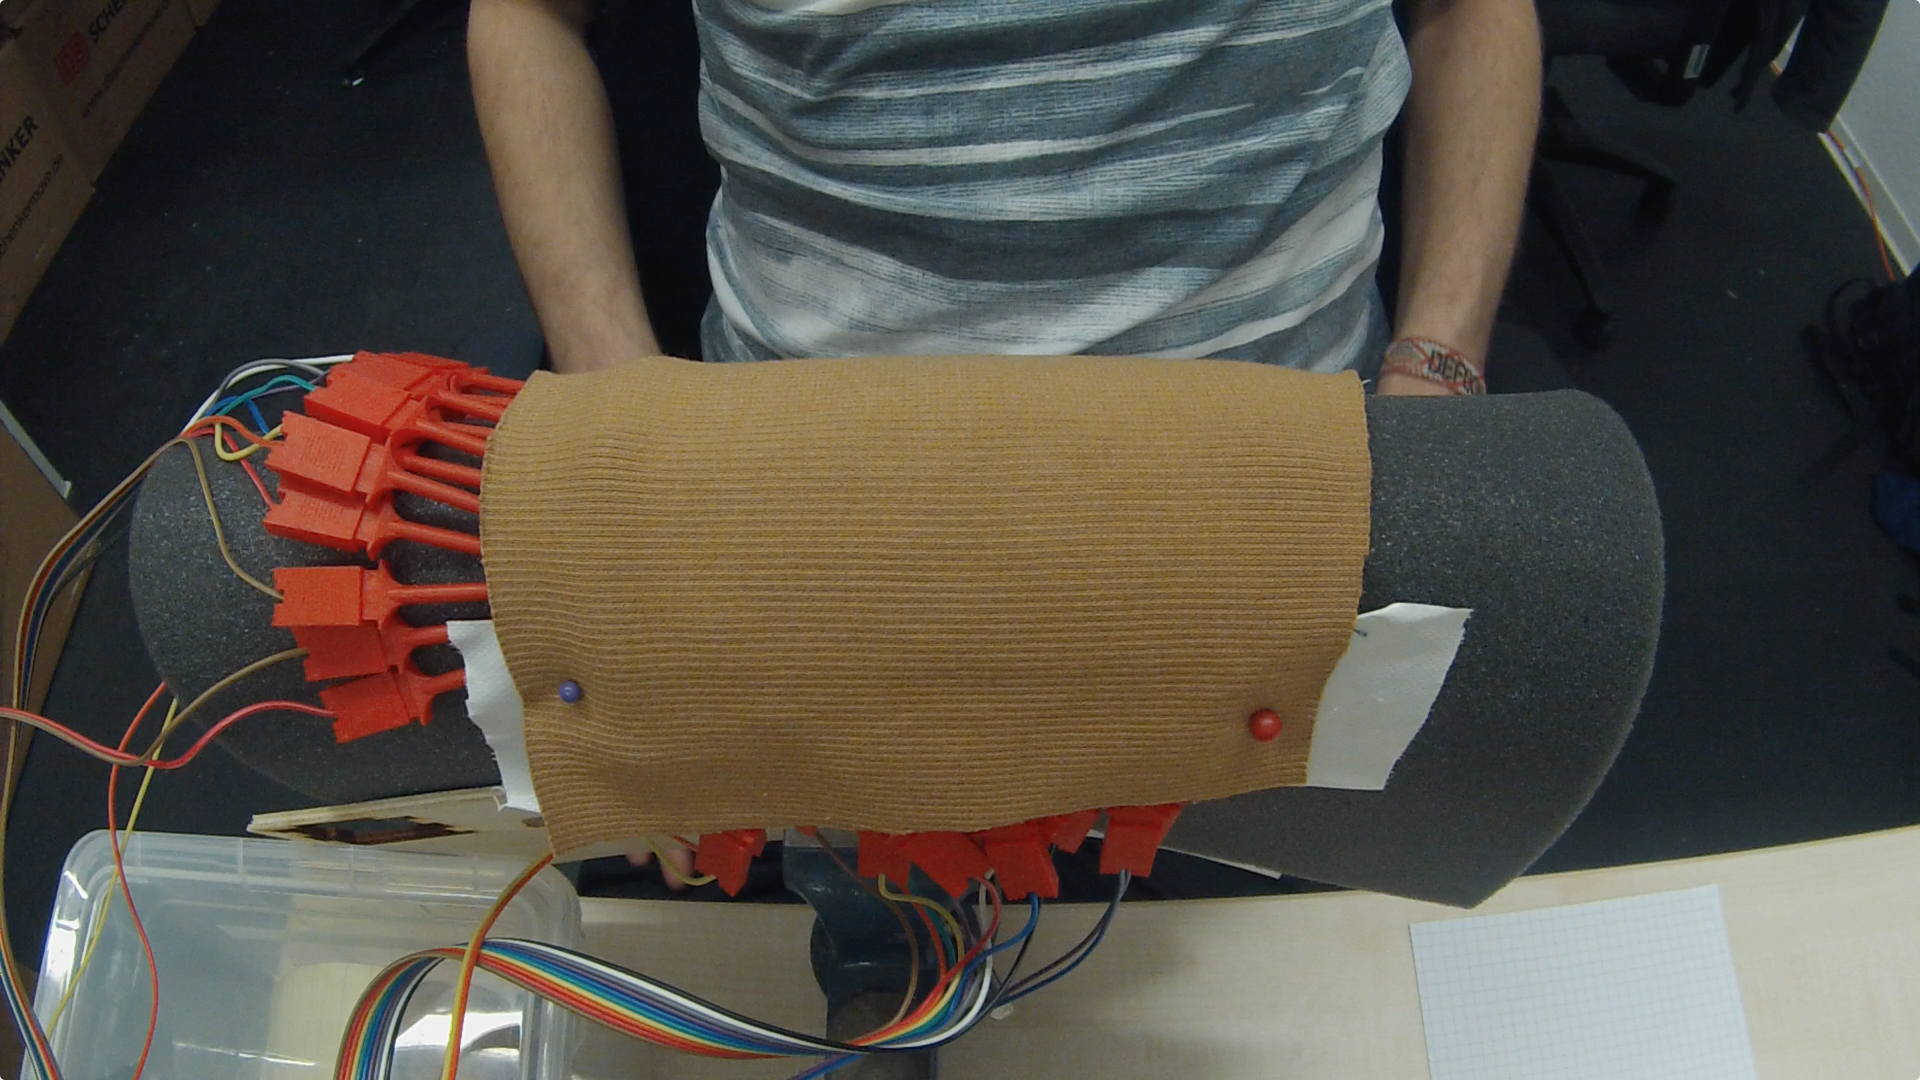
\includegraphics[scale=0.15]{images/53mmtopview.jpg}
\caption{Condition: 53mm, rib knit fabric, foam, hemmed in  a vise}
\label{fig:53mmtopview}
\end{figure}\mnote{Study design and participants}We asked two right-handed participants, one male (24) and one female (22) to test our prototype. One had no experience with wearables. The participants had to perform 8 gestures in each condition with three repetitions. We selected a within-subject design for the evaluation since we only let two users with different experience participate. Thus, each participant had to perform 423 (18 conditions + 8  gestures * 3 repetitions) gestures not including potential repetitions. The set of gestures is shown in figure \ref{fig:gestureTemplate}. Curvature and softness were counterbalanced. Since each change of a condition takes several minutes we decided to shorten the time for the participant. To do so we tested the upper fabrics consecutively. \\
\begin{center}
\begin{figure}
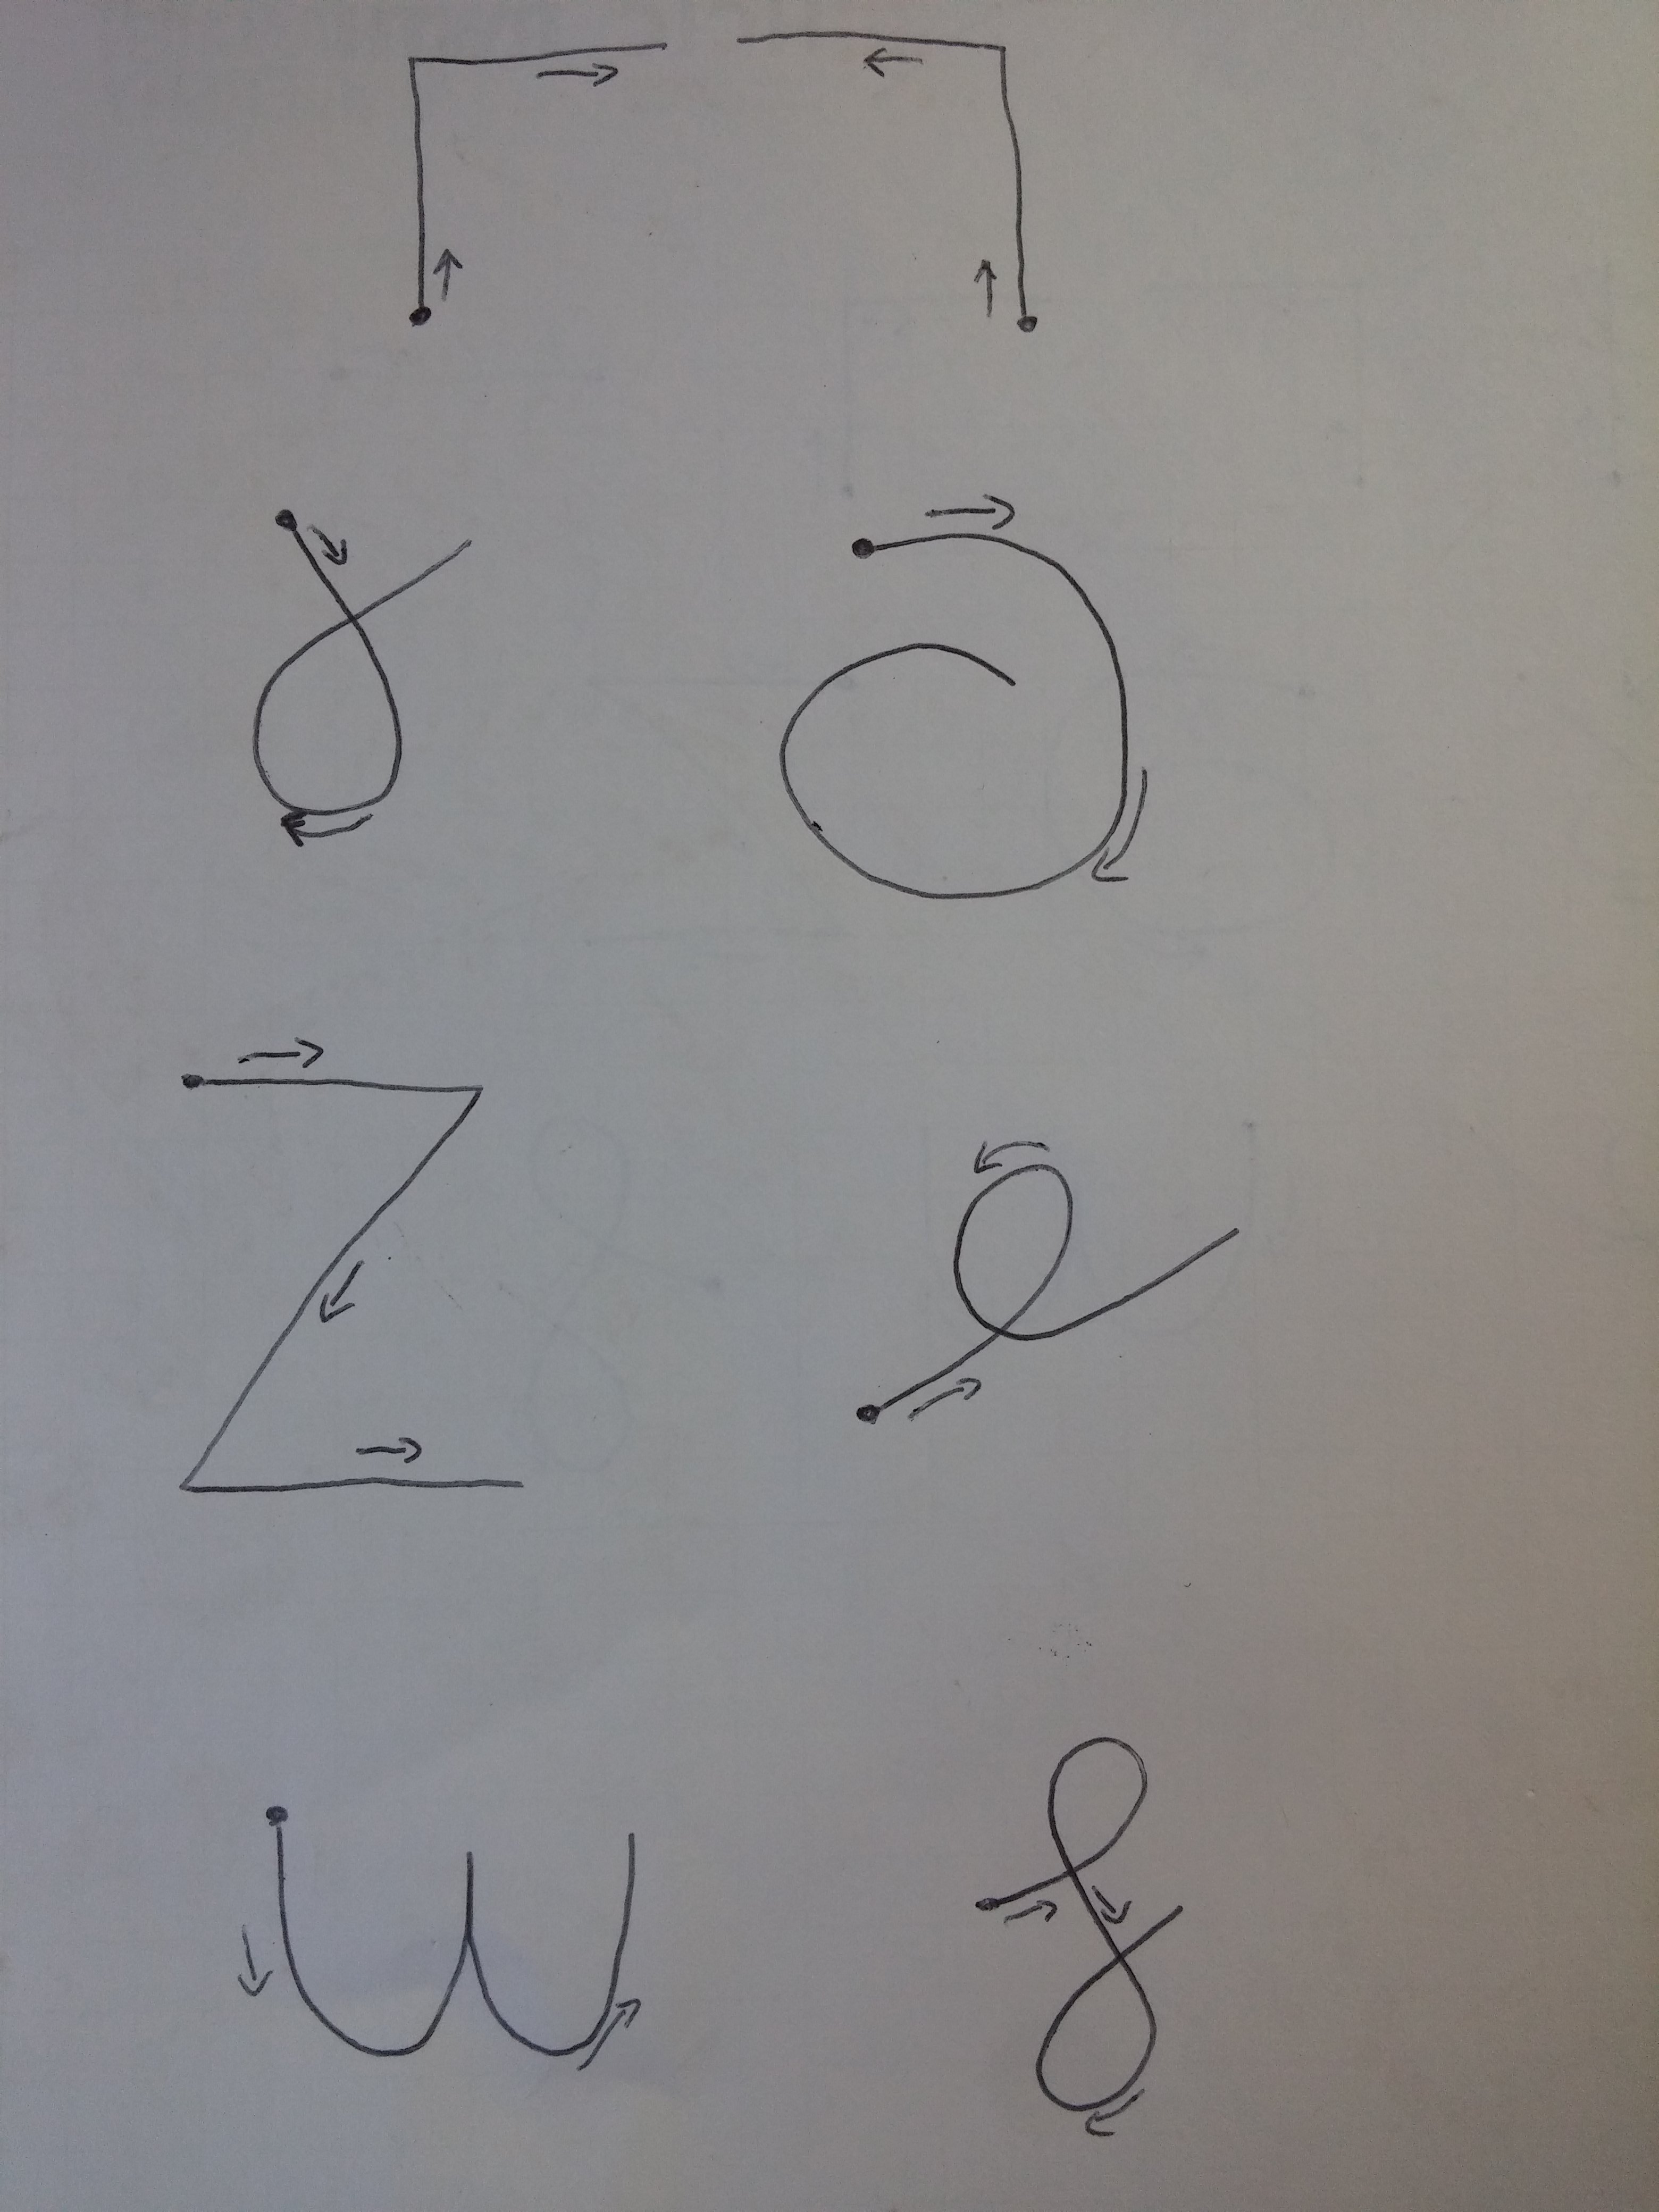
\includegraphics[scale=0.07]{images/gestureTemplate.jpg}
\caption{Gesture set: right angle, left angle, slope, spiral, z, pigtail, w, doubleslope}
\label{fig:gestureTemplate}
\end{figure}
\end{center}

\section{Study Procedure}
After the user arrived we introduced our prototype. We explained the basic functionality and demonstrated how the output looks like. Then we let the user test the eight gestures and some freestyle strokes. This was done without foam or any additional fabric. We pointed out that a certain amount of pressure is essential for our prototype to recognize the touch. When they felt familiar enough, about 2 minutes of testing, we prepared the first condition. 
\\ \\
For each condition we setup a GoPro Hero 3 to capture the prototype and the acting hand of the user. When we were ready to start recording the screen and setup, we told the user to continue. Since the user cannot see the output during the study, we told the user when insufficient  pressure was applied or when the touch-sensing area was left. In both cases we most likely recognized one or two wrong gestures. We represent the number of wrong gestures with an \emph{x} in the respective chart. 
\\ \\
When one condition is completed we asked the user about their impressions of the fabric, softness, and curvature. 

\section{Observation}
The results proof the general applicability of our prototype. The overall success rate of performed gesture is shown in figure \ref{fig:overallRecognition}. We distinguish between the hardware results by eye, with recognition, \mnote{Distinguish between hardware and gesture recognition}and with repetition if the user left the touch sensing area. 84.5\% of all gestures generated recognizable data. Meaning that by eye the output of the data matches the current gesture. However only 75.5\% of these gestures were recognized correctly using the 1\$ recognizer.  One example of a false negative is shown in figure~\ref{fig:falsenegative}. We made this separation, since we are primarily interested in the capabilities of our hardware prototype. \\
Additionally, we let the participants repeat those trials, where they  left the touch sensing area. This leads to an average success rate of 87.5\% and the second user even achieved 91\%.
\begin{figure}
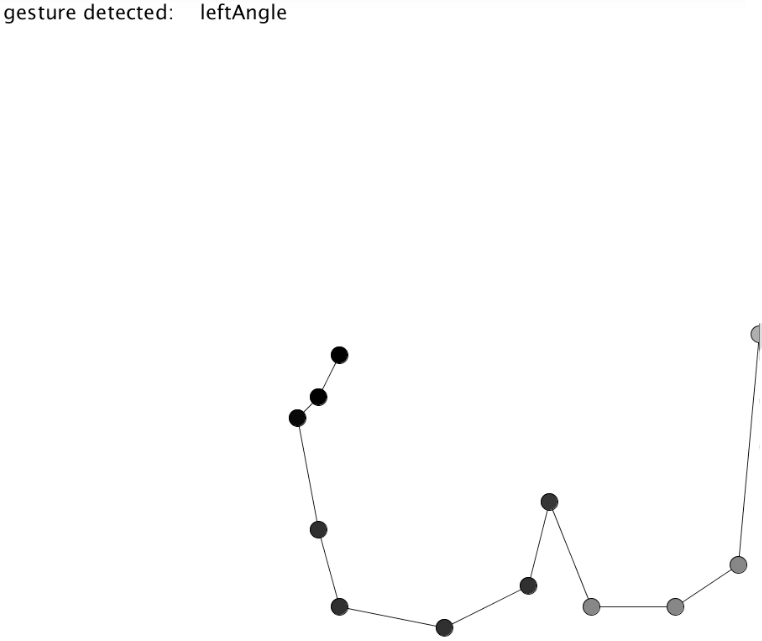
\includegraphics[scale=0.35]{images/falsenegative.jpg}
\caption{The characteristics of \emph{w} are there, but nonetheless \emph{leftAngle} was detected.}
\label{fig:falsenegative}
\end{figure}
\begin{figure}
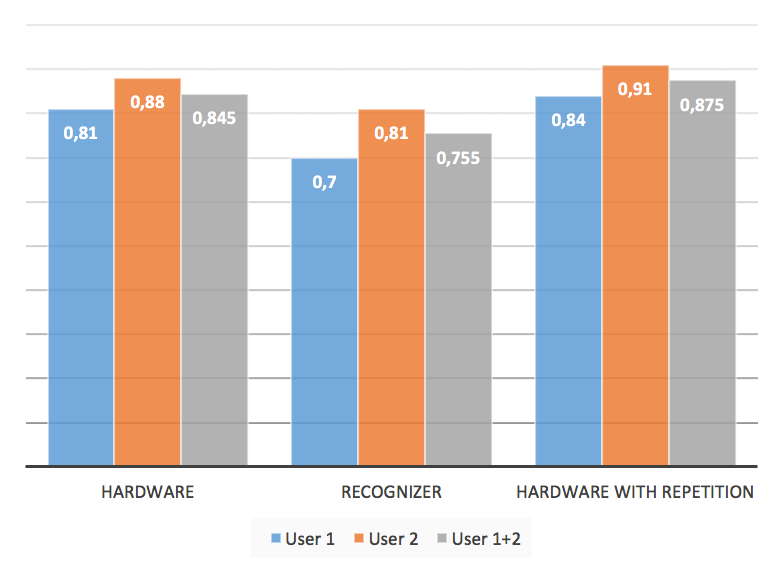
\includegraphics[scale=0.35]{images/overallRecognition.jpg}
\caption{Success rate of all performed gestures with different criteria.}
\label{fig:overallRecognition}
\end{figure}
\\
The difference of hardware success rate and recognizer success rate is almost the same for all conditions. Since we are interested in the performance of the hardware we only consider the success rate of the hardware from now on. \\ \\
\mnote{Flat surface is best and 53mm worst}When it comes to surface curvature we got the results we expected shown in figure \ref{fig:surface}. The curvature with a 53mm diameter performs worst but still with a success rate of 75.5\%. The best curvature is no curvature at all. On the table both users achieved a success rate above 90\% with an average of 92\%. It is notable that the user with experience obtained a rate of 95\% with 66mm curvature where the other user got 79\%. Nevertheless, the inexperienced user outperformed the other user on the flat surface. 
\\
When we asked the participants which curvature they prefer they agree that the flat surface is most pleasant for touch input and the more curvature, the more likely it happens that they slip off the surface. This leads to unintentional input and thus to more input error. 
\begin{figure}
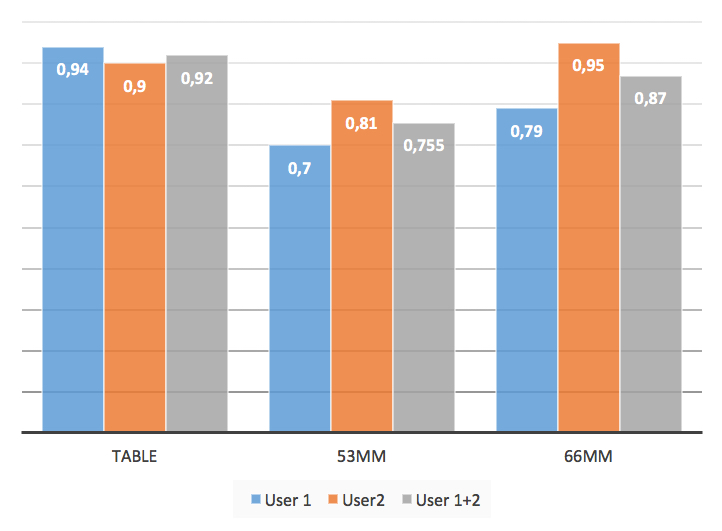
\includegraphics[scale=0.35]{images/surface.jpg}
\caption{Success rates on surface curvatures}
\label{fig:surface}
\end{figure}
The success rates with different softness are shown in figure \ref{fig:foam}. \mnote{Only slight improvement with foam}Our hypothesis  that softness has a bad influence on the performance of our prototype was falsified. One user obtained 81\%  in both cases and the more experienced user performed better on the foam (92\%). The participants reported that is was much more pleasant to perform the gestures on the foam due to the distribution of the pressure. 
\\ \\
\begin{center}
\begin{figure}
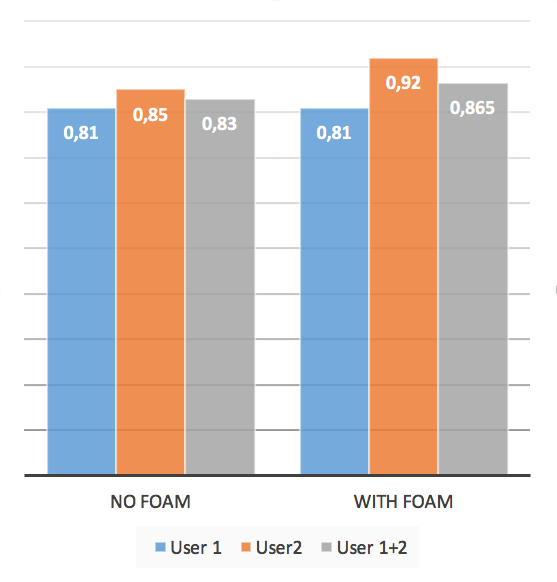
\includegraphics[scale=0.5]{images/foam.jpg}
\caption{Success rates with and without foam}
\label{fig:foam}
\end{figure}
\end{center}
The different materials seem to have no influence on the performance of our prototype as shown in figure \ref{fig:materials}. The average success rate is between 84\% and 86\%. However, the participants reported that the rib knit fabric is extremely annoying due to the immense flexibility. One user said he likes jeans for getting good results but after a while the abrasive surface of the jeans leads to tingle and makes it unpleasant. Both participant prefer cotton and jeans because of their stiffness resulting in less folds. Although the participants reported occasional wrinkles of the rib knit fabric and therefore perceived lose of contact, the sensor still recognized the input as fine as the other fabrics. 
\\ \\
\begin{center}
\begin{figure}
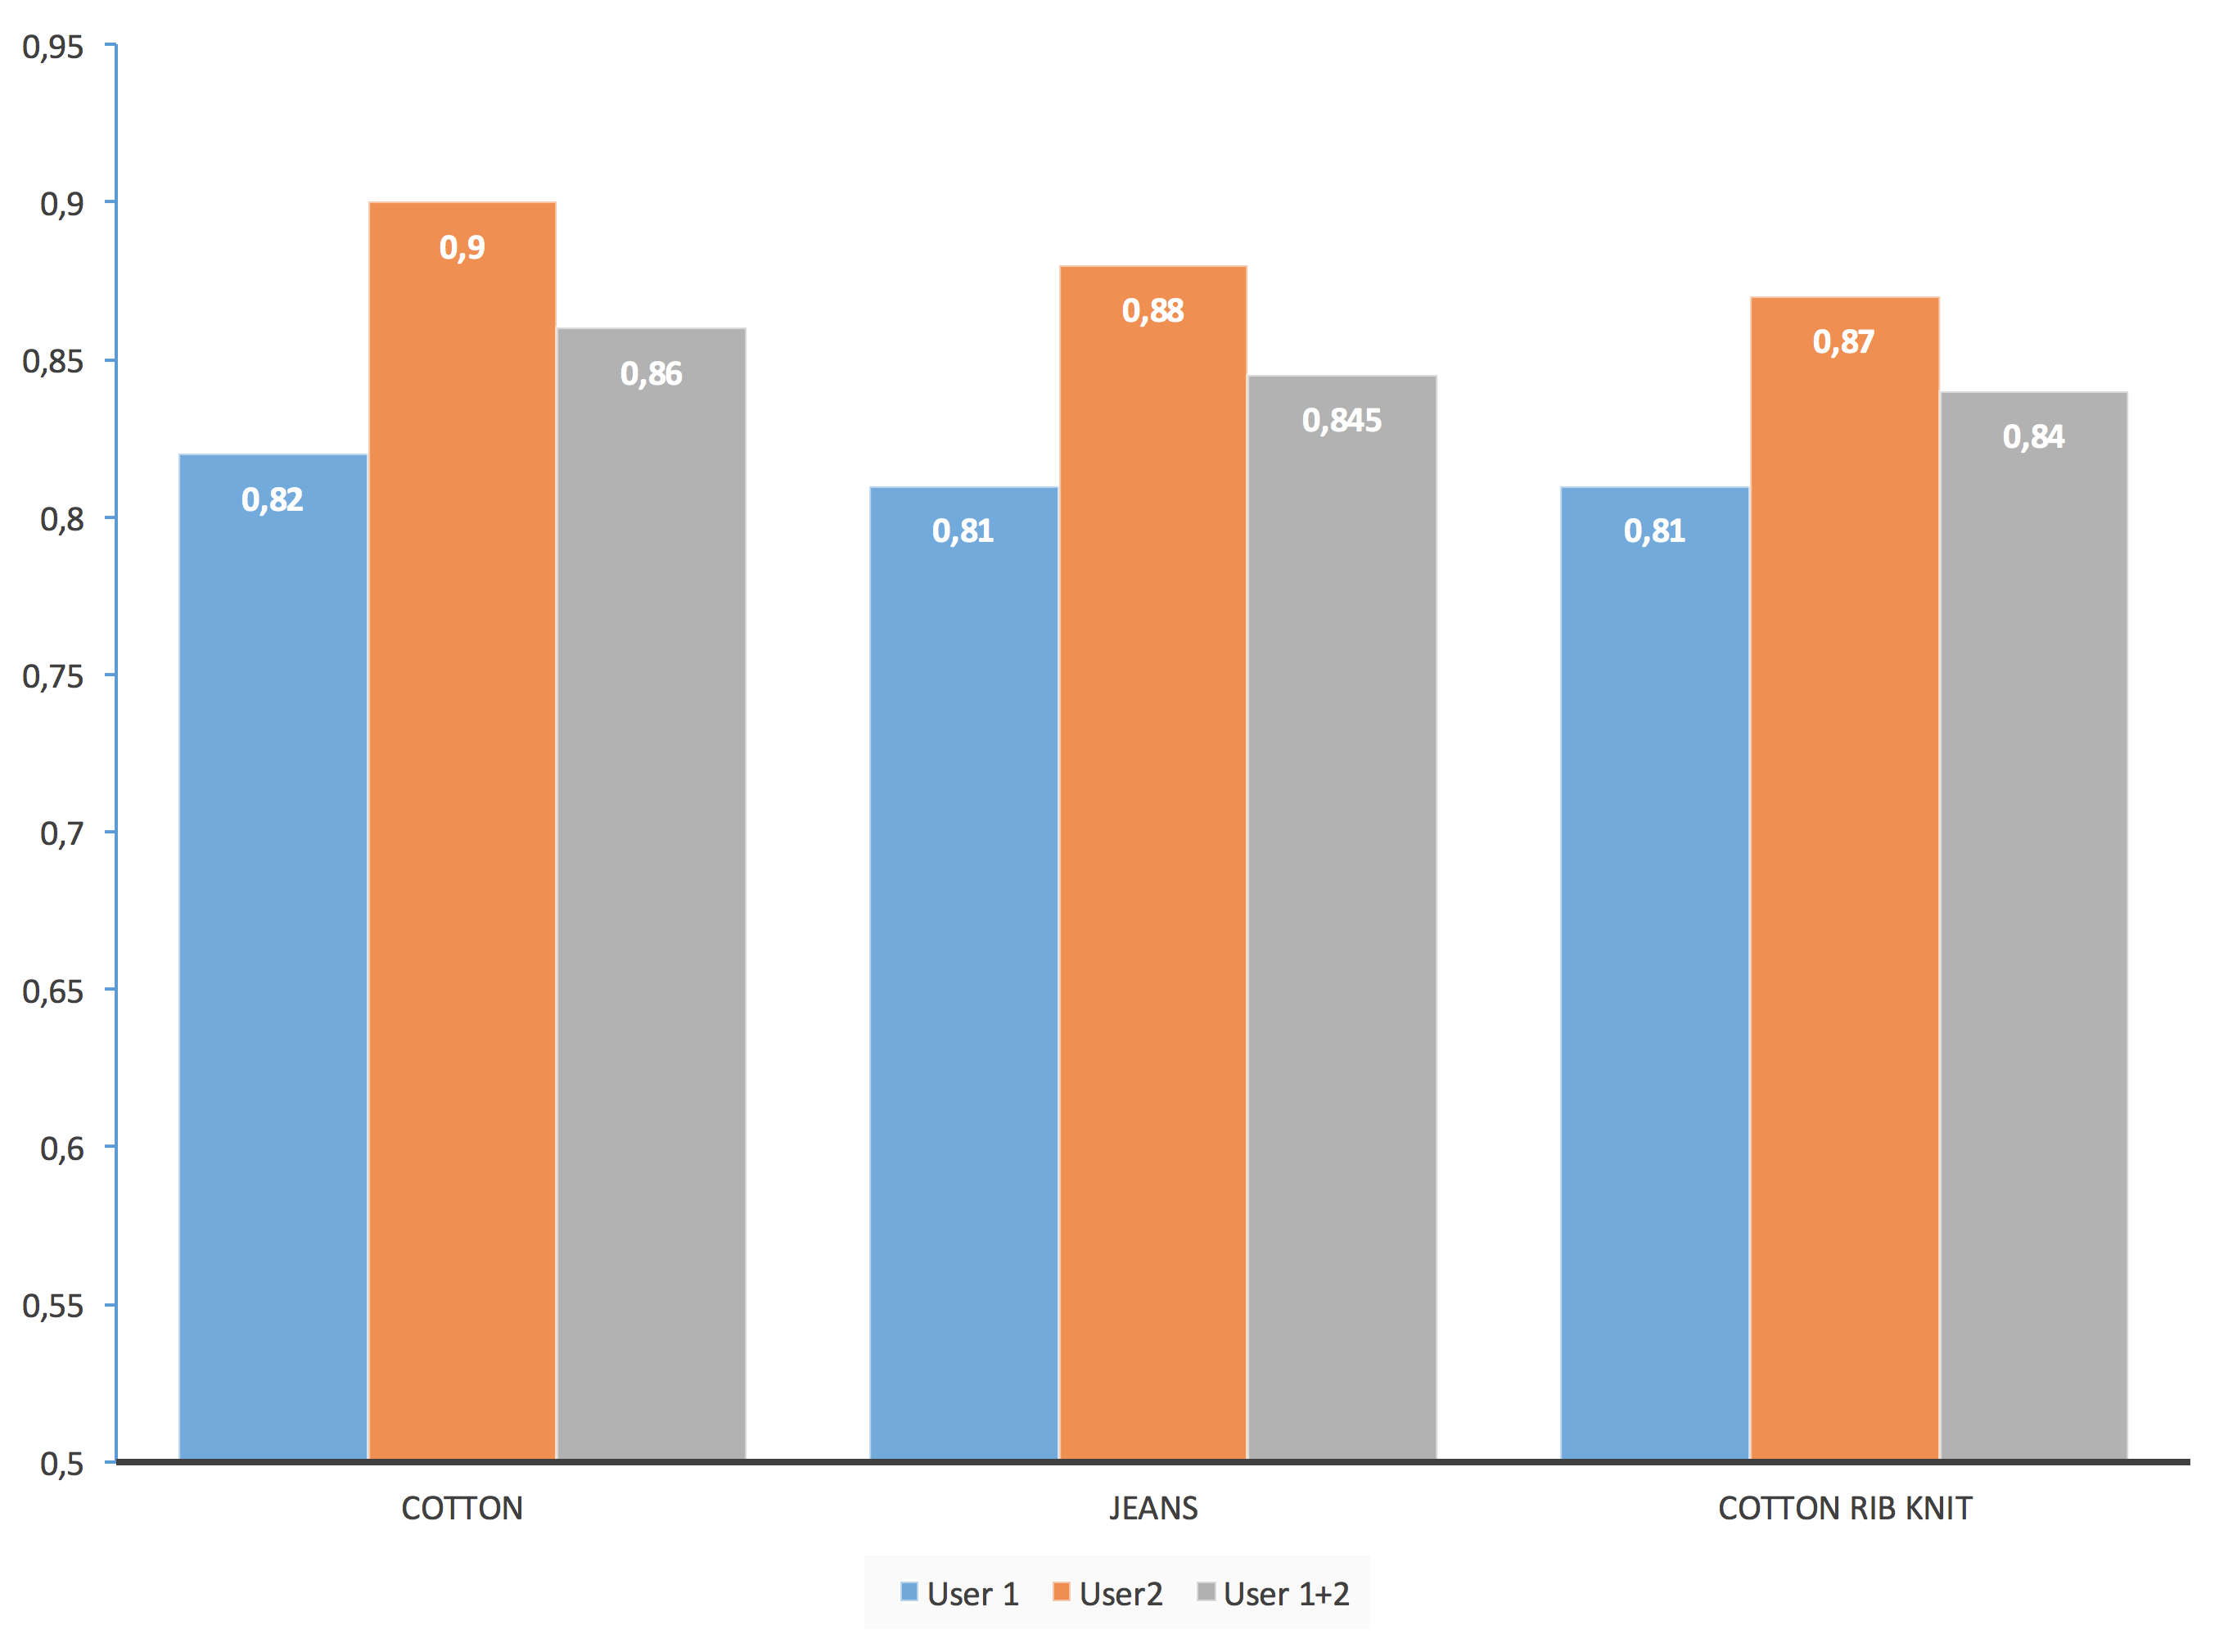
\includegraphics[scale=0.4]{images/materials.jpg}
\caption{Success rates with different materials}
\label{fig:materials}
\end{figure}
\begin{figure}
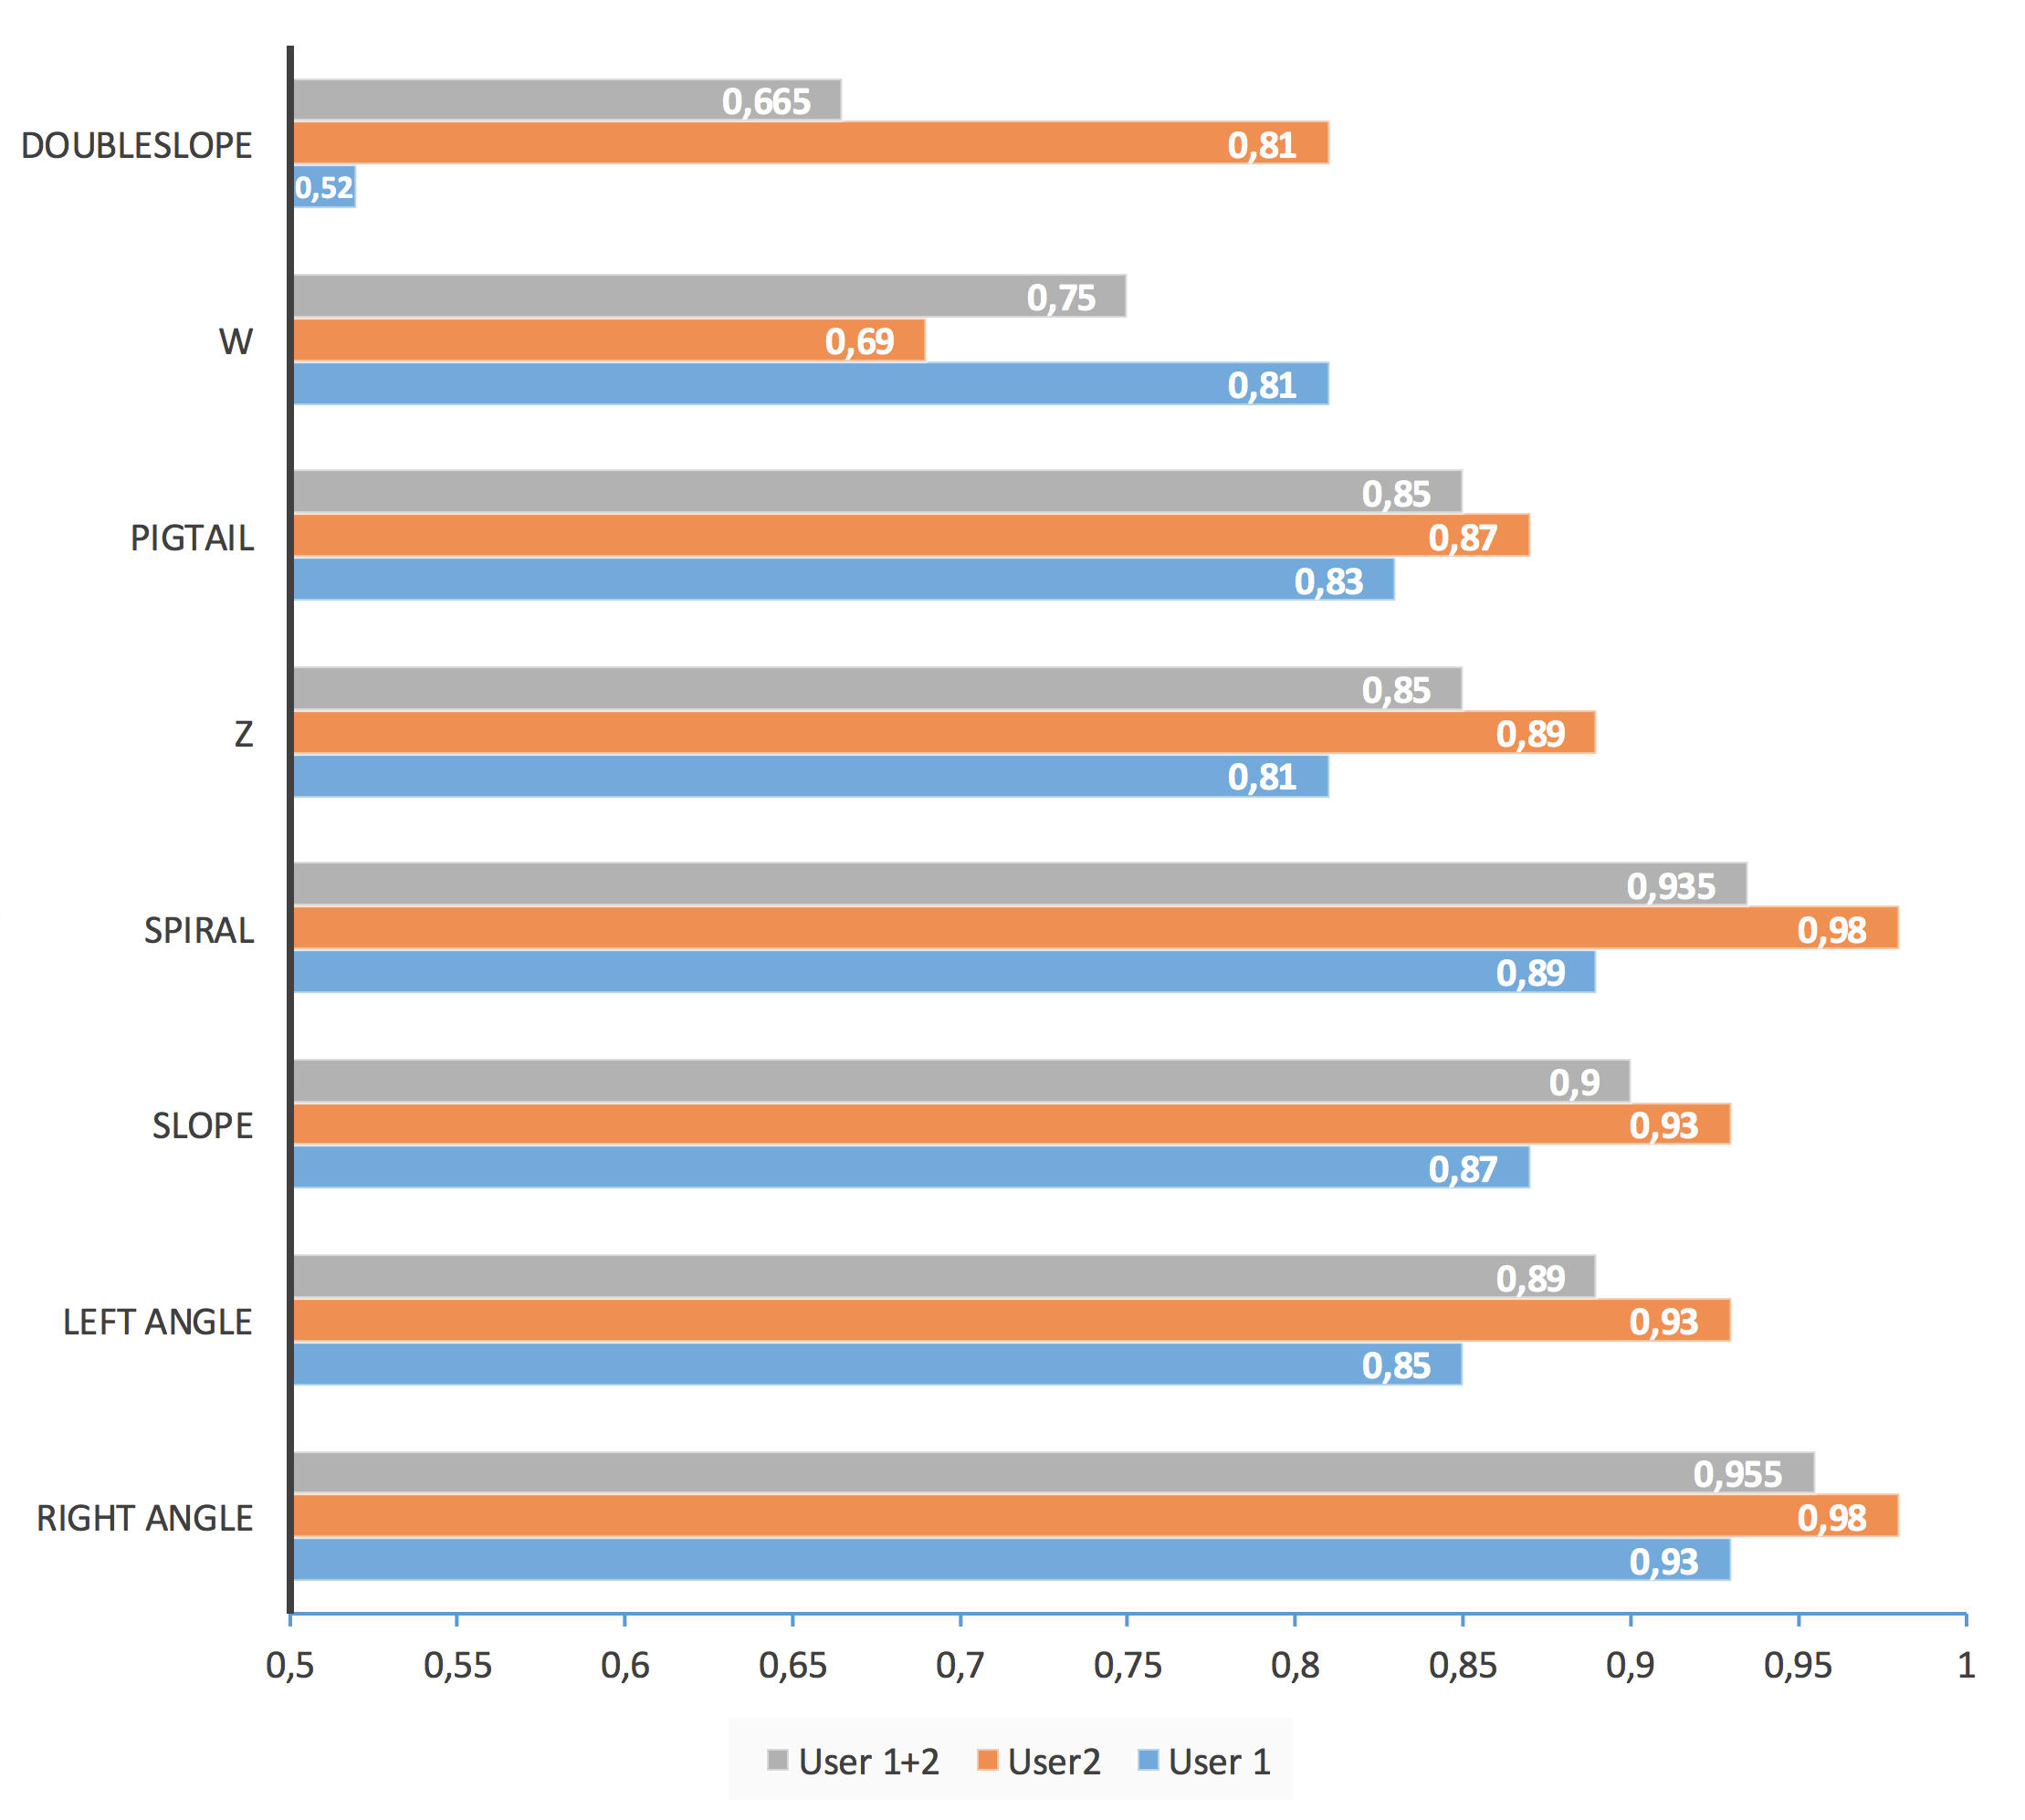
\includegraphics[scale=0.4]{images/gestures.jpg}
\caption{Success rates for each gesture}
\label{fig:gestures}
\end{figure}
\end{center}
The success rates of each gesture are shown in figure \ref{fig:gestures}. The most complex gesture was \emph{doubleslope} and was the hardest gesture to perform with an average success rate of 66.5\%. However the difference between the users is huge (81\% and 52\%). Applying the required amount of pressure steadily is more difficult when the gesture key characteristics are complex. The \emph{doubleslope} gesture requires more changes of direction than \emph{pigtail} (average 85\%).
\\
There is notable difference between \emph{left angle} (89\%) and \emph{right angle}, which has the best  average success rate of 95.5\%. It remains to test if this is ascribed to the dominant hand. Except for the \emph{w} gesture (75\%), the rest of the gestures are within 85\% and 93.5\%. 

\section{Conclusion}
The surface curvature has the most meaningful effect on the performance of the prototype next to the characteristics of a gesture. There is a consistent difference between the two participants due to the varying level of experience. This indicates a learning effect which also was the subjective estimation of both participants. Primarily the required pressure to generate a contact is remembered over time. 